\chapter{状态方程、辐射与真空能}

\lectureoverview{均匀宇宙的历史在很大程度上就是其标度因子\(a(t)\)的历史。弗里德曼方程给出了几何，但物质的状态方程告诉我们空间膨胀时能量密度如何变化。我们首先由流体所做的功导出\(\rho\propto a^{-3(1+w)}\)，然后通过计算光子动量转移得到辐射的\(P=\rho/3\)，最后通过\(P=-\rho\)来确认真空能。正的真空能产生德西特膨胀；曲率与宇宙学常数的符号则产生反弹与再坍缩解，这些解可以读作简单的力学系统。}

\section{标度因子与缺失的物质定律}

让我们先回顾一下我们要走向何处。在均匀且各向同性的近似下，主要的宇宙学历史被编码在一个函数\(a(t)\)之中。知道这个函数并不能回答关于宇宙的所有问题，但它决定了距离、膨胀速率以及大尺度各时期的先后顺序。本讲的目的还不是从观测上确立这些时期，而是从基本物理出发，导出使这些模型成为可能的状态方程。

两个基准模型已经出现过：
\begin{equation}
a(t)\propto t^{2/3}
\qquad\text{(matter domination)},
\end{equation}
以及
\begin{equation}
a(t)\propto t^{1/2}
\qquad\text{(radiation domination)}.
\end{equation}
这两条定律都不是在所有时期都精确成立。辐射给出了有用的早期近似，物质给出了较晚的中间时期近似；真空能最终又会改变晚期行为。当前的问题不是观测如何揭示这些时期，而是弗里德曼方程相应的右端项之间有何区别。

\begin{figure}[htbp]
\centering
\includegraphics[width=0.72\textwidth]{lecture_05_figure_02.png}
\caption{复习过的标度因子幂律与新引入的密度符号。这是过渡性的板书状态，而非已完成的推导。}
\label{fig:c05-review-board}
\lectureframe{00:03:18.380}
\end{figure}

缺失的桥梁是状态方程。它决定了弗里德曼方程右端的能量密度如何随标度因子变化。两条基准定律是
\begin{equation}
\rho_{\text{matter}}=\frac{\rho_0}{a^3},
\qquad
\rho_{\text{rad}}=\frac{\rho_0}{a^4}.
\label{eq:c05-benchmark-densities}
\end{equation}
物质随体积稀释，而体积按\(a^3\)标度。辐射则多下降一个\(a\)的幂次。我们希望把这两条规则都理解为压强与能量密度之间关系的推论。

\section{从压强到密度标度定律}

状态方程一般可能涉及密度、压强、温度以及其他变量。对于这里所考虑的宇宙学组分，采用有用的常数\(w\)形式
\begin{equation}
P=w\rho,
\label{eq:c05-eos}
\end{equation}
其中\(w\)表征该流体。板书用的是大写\(W\)；我们使用习惯的小写\(w\)。这种线性形式涵盖了下面几个重要情形，但它是一种简化假设，而不是所有可能流体都遵守的定律。

对于非相对论性物质，能量密度由静能主导。若\(n\)为数密度，\(m\)为粒子质量，则示意性地有
\begin{equation}
\rho\simeq nmc^2.
\end{equation}
因子\(c^2\)使得即便很小的静质量也成为巨大的能量储备；一粒尘埃的完全湮灭会释放出宏观量级的能量。相比之下，压强由粒子撞击壁面时的动量转移产生，量级为\(nmv^2\)。保龄球比乒乓球转移更多动量，但对于冷气体，所有相关速度都满足\(v\ll c\)。因此
\begin{equation}
\frac{P}{\rho}\sim\frac{v^2}{c^2}\ll1,
\qquad
w\simeq0.
\label{eq:c05-dust-eos}
\end{equation}
辐射以\(c\)运动，因此不会共享这一近似。我们将导出其\(w\)值，而不是假设它。

我们现在需要一个通用的机器，把方程~\eqref{eq:c05-eos}转化为\(\rho\)的标度定律。一个实验室盒子就足够了。星系不能真的被放进盒子里，但经过粗粒化后它们表现得像粒子，而能量与压强之间的关系可以在局部导出。

\begin{figure}[htbp]
\centering
\includegraphics[width=0.86\textwidth]{lecture_05_figure_03.png}
\caption{状态方程、复习过的密度标度关系以及热力学盒子在同一块黑板上。讲师遮住了部分早先的书写，因此该图像用于展示布局和可见方程，而非作为完整转录。}
\label{fig:c05-box-board}
\lectureframe{00:13:39.612}
\end{figure}

黑板左侧是复习过的宇宙学标度关系；右侧开始盒子论证。合起来看，可见内容把
\begin{equation}
\rho_{\text{matter}}=\frac{\rho_0}{a^3},
\qquad
\rho_{\text{rad}}=\frac{\rho_0}{a^4},
\qquad
P=w\rho.
\end{equation}
联系起来。我们的任务是从状态方程导出这两条密度定律。

一面墙的面积为 \(A\)。将其向外移动 \(dx\)，因此
\begin{equation}
dV=A\,dx.
\end{equation}
压强是单位面积上的力，所以作用在墙上的力为 \(PA\)。气体做功 \(PA\,dx=P\,dV\)，而内部剩余的能量减少。
\begin{equation}
dE=-P\,dV.
\label{eq:c05-work-law}
\end{equation}
\begin{figure}[htbp]
\centering
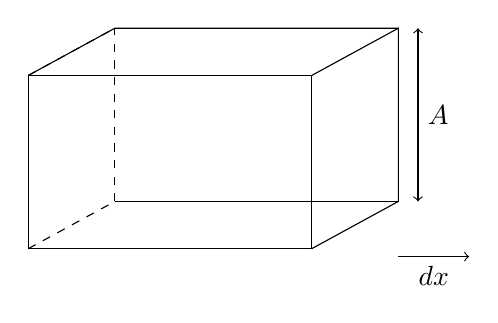
\begin{tikzpicture}[scale=1.0]
\draw (0,0) -- (3.6,0) -- (3.6,2.2) -- (0,2.2) -- cycle;
\draw (3.6,0) -- (4.7,0.6) -- (4.7,2.8) -- (3.6,2.2);
\draw (0,2.2) -- (1.1,2.8) -- (4.7,2.8);
\draw (1.1,0.6) -- (4.7,0.6);
\draw[dashed] (0,0) -- (1.1,0.6);
\draw[dashed] (0,2.2) -- (1.1,2.8);
\draw[dashed] (1.1,0.6) -- (1.1,2.8);
\draw[<->] (4.95,0.6) -- (4.95,2.8);
\node[right] at (4.95,1.7) {\(A\)};
\draw[->] (4.7,-0.1) -- (5.6,-0.1);
\node[below] at (5.15,-0.1) {\(dx\)};
\end{tikzpicture}
\caption{热力学盒子的清晰重绘，其面面积为 \(A\)，位移为 \(dx\)。}
\label{fig:c05-box-redraw}
\end{figure}

总能量为
\begin{equation}
E=\rho V.
\end{equation}
求导得
\begin{equation}
d(\rho V)=\rho\,dV+V\,d\rho.
\end{equation}
代入方程~\eqref{eq:c05-work-law}得
\begin{equation}
\rho\,dV+V\,d\rho=-P\,dV.
\end{equation}
代入 \(P=w\rho\)：
\begin{equation}
V\,d\rho=-(1+w)\rho\,dV.
\end{equation}
这个结果只是通向有用方程的前奏，但还差一点。除以 \(\rho V\)。
\begin{equation}
\frac{d\rho}{\rho}=-(1+w)\frac{dV}{V}.
\end{equation}
\begin{figure}[htbp]
\centering
\includegraphics[width=0.78\textwidth]{lecture_05_figure_04.png}
\caption{分离后的密度—体积方程以及对数积分的开头。完整的右端由前面的代数重建，而不是来自隐藏的像素。}
\label{fig:c05-log-board}
\lectureframe{00:15:35.600}
\end{figure}

画面显示了分离后的方程以及开头 \(\log\rho=\)。直接完成积分：
\begin{equation}
d(\log\rho)=-(1+w)\,d(\log V),
\end{equation}
于是
\begin{equation}
\log\rho=-(1+w)\log V+\text{const.}
\end{equation}
取指数，
\begin{equation}
\rho\propto V^{-(1+w)}.
\end{equation}
这就是密度—体积定律。

现在从盒子回到宇宙学。只移动一面墙是一种方便的推导，而不是各向异性的假设。均匀地膨胀三个方向会给出相同的做功关系，而共动体积按如下方式缩放：
\begin{equation}
V\propto a^3.
\end{equation}
因此
\begin{equation}
\boxed{\rho\propto a^{-3(1+w)}}.
\label{eq:c05-density-scaling}
\end{equation}
在 \(d\) 个空间维度中，指数 \(3\) 将变为 \(d\)；论证的其余部分不变。

\section{首批应用：物质与辐射}

我们现在可以把复习公式作为推论而不是假设重新得到。

对于非相对论性物质，我们取
\begin{equation}
w=0.
\end{equation}
于是
\begin{equation}
\rho\propto a^{-3},
\end{equation}
这正是物质稀释定律。

对于辐射，暂时取
\begin{equation}
w=\frac13.
\end{equation}
如果这是正确的，那么
\begin{equation}
\rho\propto a^{-3(1+1/3)}=a^{-4}.
\end{equation}
因此，额外的负幂等价于 \(w=1/3\)。尚未解决的步骤是从光子物理推导出该值。

\section{为什么辐射压是其能量密度的三分之一}

辐射可以描述为电磁波，也可以描述为无质量粒子。使用光子并计算盒子中光子气体的压强。盒子画成二维，但气体及其角分布是三维的。光子以光速运动，并从临时的壁上弹性反弹。

暂时假设所有光子都具有相同的能量 \(\epsilon\)。当把来自不同能量的贡献相加时，这一简化将消失。令 \(\vec{\pi}\) 为光子动量矢量；避免使用通常的 \(p\)，因为 \(P\) 已经表示压强。无质量粒子满足以下关系。
\begin{equation}
\epsilon=c\,\pi,
\end{equation}
其中 \(\pi=|\vec{\pi}|\)。在讲座所用的单位中，\(c=1\)，所以
\begin{equation}
\epsilon=\pi.
\end{equation}
如果 \(\nu\) 是光子数密度，那么能量密度为
\begin{equation}
\rho=\epsilon\,\nu.
\end{equation}
令 \(x\) 轴垂直于一面墙。在短时间间隔 \(\Delta t\) 内，一个与该法线成角 \(\theta\) 运动的光子，只有当它起始于厚度为
\begin{equation}
\Delta x=\Delta t\cos\theta.
\end{equation}
的薄层内时才能到达该墙。如果它发生反射，其动量的 \(x\) 分量反号，因此传递给墙的动量为
\begin{equation}
\Delta \pi_x=2\epsilon\cos\theta.
\end{equation}
力是单位时间内的动量传递，所以一次碰撞贡献 \(\Delta \pi_x/\Delta t\)。薄层中的光子数为 \(\nu A\Delta x\)，但其中只有一半朝墙运动，因此相关的数目是 \(\tfrac12 \nu A\Delta x\)。将总力除以墙面积 \(A\)，我们得到
\begin{align}
P(\theta)
&=
\frac{1}{A}
\left(\frac{2\epsilon\cos\theta}{\Delta t}\right)
\left(\frac12 \nu A\Delta x\right) \\
&=
\epsilon\nu\cos\theta\frac{\Delta x}{\Delta t} \\
&=
\epsilon\nu\cos^2\theta \\
&=
\rho\cos^2\theta.
\end{align}
结果依赖于角度，因为它只是沿一个方向运动的光子的贡献。

\begin{figure}[htbp]
\centering
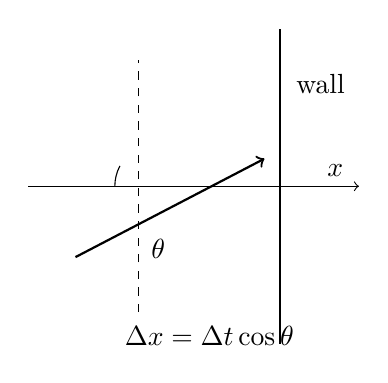
\begin{tikzpicture}[scale=1.0]
\draw[thick] (0,0) -- (0,4);
\draw[->] (-3.2,2) -- (1.0,2);
\node[above] at (0.7,2) {\(x\)};
\draw[dashed] (-1.8,0.4) -- (-1.8,3.6);
\node[below] at (-0.9,0.35) {\(\Delta x=\Delta t\cos\theta\)};
\draw[->,thick] (-2.6,1.1) -- (-0.2,2.35);
\node[below] at (-1.55,1.45) {\(\theta\)};
\draw (-2.1,2) arc[start angle=180,end angle=152,radius=0.55];
\node[right] at (0.08,3.3) {wall};
\end{tikzpicture}
\caption{以角度 \(\theta\) 入射到墙上的光子动量，这是用于推导辐射压的几何构型。}
\label{fig:c05-photon-pressure}
\end{figure}

对各项同性分布求平均。令 \(\mathbf n=(n_x,n_y,n_z)\) 为沿光子方向的单位矢量。于是
\begin{equation}
n_x=\cos\theta,
\qquad
n_x^2+n_y^2+n_z^2=1.
\end{equation}
在各向同性气体中，\(n_x^2\)、\(n_y^2\) 和 \(n_z^2\) 的平均值相等。对上述恒等式求平均，
\begin{equation}
\langle n_x^2\rangle+\langle n_y^2\rangle+\langle n_z^2\rangle=1,
\end{equation}
由对称性，每一项都相同，所以
\begin{equation}
\langle n_x^2\rangle=\langle \cos^2\theta\rangle=\frac13.
\end{equation}
因此
\begin{equation}
P=\rho\langle \cos^2\theta\rangle=\frac{\rho}{3}.
\end{equation}
所以辐射的状态方程为
\begin{equation}
P=\frac13\rho,
\qquad
w=\frac13.
\end{equation}
因子 \(1/3\) 是共享单位矢量平方的空间方向数。在 \(d\) 个各向同性空间维度中，同样的论证将给出 \(\langle n_x^2\rangle=1/d\)。这就完成了开头所承诺的微观推导。

\subsection{检验辐射论证的问题}

\begin{classroomqa}
\audiencequestion{所有光子都必须具有相同的能量吗？}
\lecturerresponse{不。在每个能量区间内分别进行计算。每个区间贡献的压强等于其自身能量密度的三分之一，因此对整个光谱求和仍保持\(P=\rho/3\)。等能量假设只是为了使记号简短。\lecturetimestamp{00:39:08--00:39:36}}
\end{classroomqa}

\begin{classroomqa}
\audiencequestion{吸收性黑壁会给出与完美镜面相同的答案吗？空无一物的空间中的壁又是什么？}
\lecturerresponse{处于热平衡的黑壁吸收并重新发射辐射，产生相同的平均动量平衡。宇宙学空间没有字面意义上的壁；该表面是一个想象出来的边界。对于每一个向外穿过的光子，各向同性都会提供一个平均的向内补偿通量，因此局域动量流的计算不变。教室中的辐射主要是热宇宙微波背景辐射，对这种辐射而言，这种平衡图像尤为自然。\lecturetimestamp{00:39:37--00:41:19}}
\end{classroomqa}

\begin{classroomqa}
\audiencequestion{量子统计会改变\(P=\rho/3\)吗？}
\lecturerresponse{不。玻色统计决定光子如何占据可用的模式，因而决定光谱和总\(\rho\)，但无质量粒子的各向同性应力仍然是该能量密度的三分之一。\lecturetimestamp{00:41:51--00:42:02}}
\end{classroomqa}

\begin{classroomqa}
\audiencequestion{如果光子彼此散射会怎样？}
\lecturerresponse{普通的光子-光子散射极其微弱，因此它在这里的修正可以忽略不计。在足够高的温度和密度下，碰撞可以产生电子-正电子对，并改变有效粒子成分和状态方程。这是一个真实的效应，但它属于比本论证所用温度高得多的区域。\lecturetimestamp{00:42:02--00:43:08}}
\end{classroomqa}

\begin{classroomqa}
\audiencequestion{壁面积\(A\)到哪里去了？}
\lecturerresponse{中间乘积是一个光子施加的力乘以撞击壁的光子数，而该光子数与\(A\)成正比。压强是力除以面积，因此最后的除法消去了\(A\)。过早地把中间表达式称为压强是板书中的疏漏；恢复从力到压强的这一步即可修正。\lecturetimestamp{00:43:11--00:44:01}}
\end{classroomqa}

\section{负压强与张力的含义}

到目前为止，粒子撞击壁并将壁向外推。这一图像自然产生正压强，但它并未穷尽所有可能性。

\begin{classroomqa}
\audiencequestion{能量密度本身可以为负吗？}
\lecturerresponse{量子理论在受限情形下允许负能量密度，而宇宙学常数在形式上可以取任一种符号。这类情形需要谨慎处理，并非直接的出发点。更熟悉的入口是负\emph{压强}，它甚至可以在能量密度为正时出现。\lecturetimestamp{00:44:25--00:44:59}}
\end{classroomqa}

\begin{classroomqa}
\audiencequestion{压强如何能为负？}
\lecturerresponse{在一维世界中，盒子是一个线段。自由运动的粒子从两端弹回并向外推，给出正压强。改为用一根拉伸的弦或弹簧连接两端。把两端拉开会使弹簧将它们向内拉。这个向内的力就是张力，即负压强的一维模型。\lecturetimestamp{00:45:04--00:46:31}}
\end{classroomqa}

\begin{figure}[htbp]
\centering
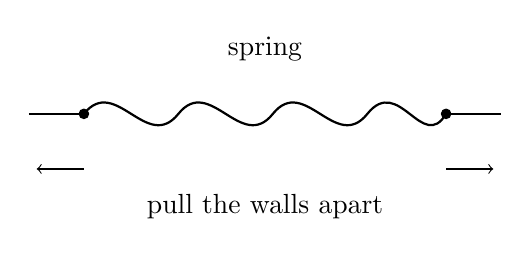
\begin{tikzpicture}[scale=1.0]
\draw[thick] (-3,0) -- (-2.3,0);
\draw[thick] (2.3,0) -- (3,0);
\draw[fill] (-2.3,0) circle (0.06);
\draw[fill] (2.3,0) circle (0.06);
\draw[thick] (-2.3,0)
.. controls (-1.9,0.5) and (-1.5,-0.5) .. (-1.1,0)
.. controls (-0.7,0.5) and (-0.3,-0.5) .. (0.1,0)
.. controls (0.5,0.5) and (0.9,-0.5) .. (1.3,0)
.. controls (1.7,0.5) and (2.0,-0.5) .. (2.3,0);
\draw[->] (-2.3,-0.7) -- (-2.9,-0.7);
\draw[->] (2.3,-0.7) -- (2.9,-0.7);
\node[below] at (0,-0.9) {pull the walls apart};
\node[above] at (0,0.55) {spring};
\end{tikzpicture}
\caption{一维弹簧作为负压强的类比。}
\label{fig:c05-tension}
\end{figure}

功的记账也相应地反转。膨胀让正压强的气体做功并损失内能。向外拉拽以对抗张力则将能量储存在弹簧中。更一般地，相互吸引的成分可以彼此拉拽，并把边界向内拉。因此，一个系统可以具有\(\rho>0\)和\(P<0\)，从而给出\(w<0\)，而没有任何矛盾。这一可能性至关重要，因为真空能量恰好具有这样的符号模式。

\section{真空能与宇宙学常数}

真空能量被赋予空无一物的空间本身。量子场论通过与场模式相联系的谐振子的零点运动来为其提供依据，但其宏观描述并不要求我们解决那个微观问题。其定义性性质是：无论选择多大的区域、无论该区域位于何处，空无一物的空间都具有相同的能量密度。
\begin{equation}
\rho=\rho_0=\text{const.}
\label{eq:c05-vacuum-density}
\end{equation}
如果一个体积为\(V\)的区域只包含真空能量，那么该区域中的总能量为
\begin{equation}
E=\rho_0 V.
\end{equation}
\begin{classroomqa}
\audiencequestion{盒子是否会通过限制允许的场模式而改变真空密度？}
\lecturerresponse{有限区域中的总能量小于整个空间中的能量，因为该区域的体积更小；体密度\(\rho_0\)保持不变。真实的边界可以改变模式能量并产生卡西米尔效应，但这种修正只有在间距与相关波长可比时才会起作用。它不是宇宙学中所使用的宏观尺度真空密度。\lecturetimestamp{00:50:06--00:51:25}}
\end{classroomqa}

引入
\begin{equation}
\Lambda=\frac{8\pi G}{3}\rho_0.
\label{eq:c05-lambda-definition}
\end{equation}
这一定义吸收了弗里德曼方程中出现的组合。其逆关系为
\begin{equation}
\rho_0=\frac{3\Lambda}{8\pi G}.
\end{equation}
参数\(\Lambda\)是宇宙学常数。一个驱动晚期加速的正的、近乎恒定的成分通常被称为暗能量。

标度因子的依赖关系已经确定，因此将盒子论证反向运行以发现其压强。由于\(d\rho_0=0\)，
\begin{equation}
dE=d(\rho_0V)=\rho_0\,dV.
\end{equation}
另一方面，热力学功关系仍然是
\begin{equation}
dE=-P\,dV.
\end{equation}
如果我们写\(P=w\rho_0\)，那么
\begin{equation}
dE=-w\rho_0\,dV.
\end{equation}
比较可得
\begin{equation}
w=-1.
\end{equation}
因此
\begin{equation}
P=-\rho.
\end{equation}
弹簧类比正是在为此处的符号做准备。正的真空能量具有负压强；负的真空能量具有正压强。对\(w\)的天文测量追问的是：晚期成分是否真的表现为一种不稀释的真空——\(w\)越接近\(-1\)，其行为就越接近方程~\eqref{eq:c05-vacuum-density}。

\begin{classroomqa}
\audiencequestion{\(P=-\rho\)是空宇宙的状态方程吗，我们能否计算\(\rho_0\)？}
\lecturerresponse{当存在真空能量时，它是空无一物的空间的状态方程。其大小则要困难得多。每一种量子场和每一个能标都可能作出贡献，包括尚未发现的场，因此没有任何公认的计算能够解释观测值。主要的谜题不是如何写出\(w=-1\)，而是为什么净\(\rho_0\)如此极其微小。\lecturetimestamp{00:57:27--00:58:29}}
\end{classroomqa}

\section{弗里德曼动力学中的真空能量}

像我们此前分离纯物质和纯辐射那样分离真空能量。当\(\rho=\rho_0\)时，弗里德曼方程变为
\begin{equation}
\left(\frac{\dot a}{a}\right)^2=\Lambda-\frac{k}{a^2},
\label{eq:c05-vacuum-friedmann}
\end{equation}
其中\(k=+1,0,-1\)分别对应球面、平坦和双曲空间。正的与负的\(\Lambda\)，结合\(k\)的三种选择，给出六种符号情形，尽管并非每一种情形都允许实解。

\begin{remark}
本讲定义\(\Lambda=(8\pi G/3)\rho_0\)，因此这里的\(\Lambda\)具有\(H^2\)的量纲。在常见约定\(G_{\mu\nu}+\Lambda_{\mathrm E}g_{\mu\nu}=8\pi G T_{\mu\nu}\)中，相应的参数为\(\Lambda_{\mathrm E}=3\Lambda\)。
\end{remark}

\subsection{平坦德西特膨胀}

令\(k=0\)。于是
\begin{equation}
\left(\frac{\dot a}{a}\right)^2=\Lambda.
\end{equation}
对于\(\Lambda>0\)，选择膨胀分支：
\begin{equation}
\dot a=\sqrt{\Lambda}\,a,
\end{equation}
因此
\begin{equation}
a(t)=C\,e^{\sqrt{\Lambda}\,t}.
\end{equation}
哈勃参数于是为常数：
\begin{equation}
H=\frac{\dot a}{a}=\sqrt{\Lambda}.
\end{equation}
这就是平坦切片中的德西特空间，以威廉·德西特命名，他在爱因斯坦于1917年引入宇宙学常数项后不久便找到了该解。如果\(\Lambda<0\)而\(k=0\)，则方程~\eqref{eq:c05-vacuum-friedmann}没有实解，因为\(H^2\)不可能为负。

\begin{classroomqa}
\audiencequestion{这里的哈勃参数真的是常数吗，这个时空有大爆炸吗？}
\lecturerresponse{对于纯平坦切片解，\(H=\sqrt{\Lambda}\)严格为常数。尽管只有当\(t\to-\infty\)时才有\(a(t)\to0\)，但这个坐标片并非测地完备的：一些指向过去的轨迹会在有限固有时内到达其边界。因此，该公式本身并不能解决全局大爆炸问题。完整的德西特几何包含的不只是这个平坦片，这一点将推迟到详细研究该几何时再讨论。\lecturetimestamp{01:06:54--01:08:07}}
\end{classroomqa}

一个包含物质、辐射、曲率和真空能量的宇宙的示意性弗里德曼方程为
\begin{equation}
\left(\frac{\dot a}{a}\right)^2
=
\Lambda+\frac{C_m}{a^3}+\frac{C_r}{a^4}-\frac{k}{a^2}.
\label{eq:c05-mixed-friedmann}
\end{equation}
在早期，当\(a\)很小时，逆幂项占主导，真空能量可以忽略。在晚期，当\(a\)很大时，常数项\(\Lambda\)占主导。因此宇宙经历了一次转变：早期它看起来由物质或辐射主导，而晚期则趋近于类德西特行为。

指数膨胀满足\(\ddot a>0\)，因此真空主导就是加速膨胀。在过渡期间，加速不必恰好是指数式的，因为物质仍然对方程~\eqref{eq:c05-mixed-friedmann}有贡献。讲座时代的观测被描述为：宇宙正处于这种竞争之中，而不是已经处于纯粹的德西特阶段。

\section{关于真空能量的问题}

\begin{classroomqa}
\audiencequestion{如果真空能量是基态能量，它怎么可能是负的？}
\lecturerresponse{一个玻色振子模式贡献\(+\tfrac12\hbar\omega\)，而一个费米子模式则以相反的符号贡献。净真空能量是对许多场和尺度的求和，因此在总和未知之前，两种符号都有可能。这些贡献的存在是自然的；解释它们异常小的剩余量才是困难的部分。\lecturetimestamp{01:12:00--01:14:12}}
\end{classroomqa}

\begin{classroomqa}
\audiencequestion{常数\(w=-1\)是否意味着未来会发生大撕裂？}
\lecturerresponse{不。具有\(w=-1\)的宇宙学常数给出类似德西特式的指数膨胀，但不会产生被称为大撕裂的有限时间发散。那种情景属于假想的幽灵组分，其\(w<-1\)，密度随宇宙膨胀而增长。这里不假设存在这样的组分。\lecturetimestamp{01:14:13--01:15:50}}
\end{classroomqa}

\begin{classroomqa}
\audiencequestion{精确的超对称会使真空能量消失吗？}
\lecturerresponse{它可以抵消零点贡献，因为每个玻色自由度都与一个费米自由度配对。然而，自然界并未展现出精确的低能超对称：观测到的玻色子和费米子并不是质量简并的伙伴。因此，精确抵消并不能解释目前所观测到的世界中的真空能量。\lecturetimestamp{01:15:51--01:16:20}}
\end{classroomqa}

\begin{classroomqa}
\audiencequestion{自然的真空能量估计值与观测值之间的巨大差异是什么？}
\lecturerresponse{普适常数\(c\)、\(\hbar\)和\(G\)定义了普朗克单位。速度\(c\)限制了一切信号，\(\hbar\)确定了普适的量子不确定性尺度，而\(G\)将所有能量与引力耦合起来。由它们可以构造出量级为\(10^{-5}\)克的普朗克质量和量级为\(10^{-33}\)厘米的普朗克长度，从而得到大约每立方普朗克长度一个普朗克能量的普朗克能量密度。在这些单位下，讲座中引用的观测真空密度约为\(10^{-123}\)，具体指数取决于约定。谜团在于：为什么那些自然暗示着极大尺度的贡献，却留下如此微小但非零的结果。\lecturetimestamp{01:16:21--01:23:12}}
\end{classroomqa}

\begin{classroomqa}
\audiencequestion{如果预期存在真空贡献，物理学家为何会对发现非零宇宙学常数感到惊讶？}
\lecturerresponse{反复的观测改进一直继续发现与零一致的结果。那段历史助长了一种心理预期：某个未知的精确原理，也许存在于未来的量子引力理论中，强制实现了完全抵消。最终的探测推翻了这一预期。这种惊讶反映的是数十年来日益严格的零结果，而不是真空能量必须消失的推导。\lecturetimestamp{01:23:14--01:26:05}}
\end{classroomqa}

\begin{classroomqa}
\audiencequestion{观测能否确定暗能量是否随时间变化？}
\lecturerresponse{它们不能排除遥远未来发生突变，但可以比较数十亿年间的近期膨胀历史。测量\(w\)，或更一般地\(w(a)\)，可以检验密度在该区间内是否演化。讲座只报告了当时大约百分之十水平的限制；那个数字是历史性的，而持久的要点是\(w=-1\)对应于不变的密度。\lecturetimestamp{01:26:06--01:27:16}}
\end{classroomqa}

\begin{classroomqa}
\audiencequestion{在另一个空间维度数下，结果会看起来不同吗？}
\lecturerresponse{整体结构保持不变。在\(d\)个各向同性空间维度中，辐射具有\(w=1/d\)，并按照\(a^{-(d+1)}\)稀释，而洛伦兹不变的真空能量仍然具有\(w=-1\)。弗里德曼方程中的数值系数随维度改变，但稀释的物质、辐射与不稀释的真空之间的区别仍然存在。\lecturetimestamp{01:27:16--01:27:57}}
\end{classroomqa}

\section{曲率与力学类比}

\subsection{正曲率与正真空能量}

取\(k=+1\)和\(\Lambda>0\)：
\begin{equation}
\left(\frac{\dot a}{a}\right)^2=\Lambda-\frac{1}{a^2}.
\label{eq:c05-closed-vacuum}
\end{equation}
乘以\(a^2\)，
\begin{equation}
\dot a^2-\Lambda a^2=-1.
\label{eq:c05-inverted-oscillator}
\end{equation}
将\(a\)视为一个假想粒子的坐标。那么\(\dot a^2\)就是它的动能项，\(-\Lambda a^2\)是一个倒置的二次势，而总能量为\(-1\)。物理上允许的分支具有\(a\geq\Lambda^{-1/2}\)：宇宙从大尺度收缩，在极小值处静止，然后再次膨胀。

精确解为
\begin{equation}
a(t)=\Lambda^{-1/2}\cosh(\sqrt{\Lambda}\,t).
\label{eq:c05-closed-desitter}
\end{equation}
利用
\begin{equation}
\cosh(\sqrt{\Lambda}\,t)
=
\frac12\left(e^{\sqrt{\Lambda}\,t}+e^{-\sqrt{\Lambda}\,t}\right),
\end{equation}
该函数关于时间对称。在\(t=0\)处，\(a=\Lambda^{-1/2}\)；朝任一时间方向它都指数增长。因此闭合切片呈现收缩、非奇异极小值和再膨胀。它在整体上看起来与平坦指数切片不同，但两种坐标系覆盖的是同一de Sitter几何的不同部分。

\subsection{负宇宙学常数}

记\(\Lambda=-|\Lambda|\)。若\(k=+1\)，则方程~\eqref{eq:c05-vacuum-friedmann}对每个\(a\)都有负的右端，而\(H^2\geq0\)。这种纯真空类型不存在实的FRW解。

对于\(k=-1\)，
\begin{equation}
\left(\frac{\dot a}{a}\right)^2=-|\Lambda|+\frac{1}{a^2}.
\end{equation}
两边乘以\(a^2\)，
\begin{equation}
\dot a^2+|\Lambda|a^2=1.
\label{eq:c05-negative-lambda-oscillator}
\end{equation}
这是谐振子的能量方程。由于\(a\geq0\)，一个物理半周期为
\begin{equation}
a(t)=\frac{1}{\sqrt{|\Lambda|}}
\sin\!\left(\sqrt{|\Lambda|}\,t\right),
\qquad
0<t<\frac{\pi}{\sqrt{|\Lambda|}}.
\end{equation}
开放宇宙从\(a=0\)开始，达到\(a_{\max}=|\Lambda|^{-1/2}\)，然后回到大挤压。因此开放空间几何并不保证永恒膨胀；负宇宙学常数可以使其逆转。非常大的正\(\Lambda\)会把束缚结构撕裂，而大的负值则会导致迅速再坍缩。

\begin{figure}[htbp]
\centering
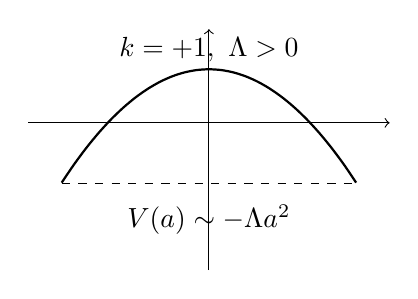
\begin{tikzpicture}[scale=0.85]
\draw[->] (-2.7,0) -- (2.7,0);
\draw[->] (0,-2.2) -- (0,1.4);
\draw[thick,domain=-2.2:2.2,smooth] plot (\x,{-0.35*(\x)^2 + 0.8});
\draw[dashed] (-2.2,-0.9) -- (2.2,-0.9);
\node at (0,-1.45) {\(V(a)\sim -\Lambda a^2\)};
\node at (0,1.1) {\(k=+1,\ \Lambda>0\)};
\end{tikzpicture}
\hspace{2em}
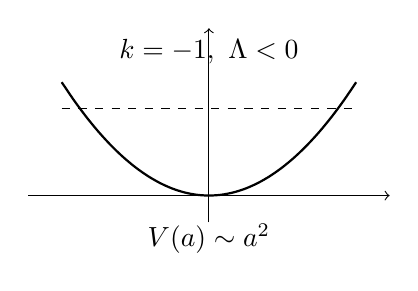
\begin{tikzpicture}[scale=0.85]
\draw[->] (-2.7,0) -- (2.7,0);
\draw[->] (0,-0.4) -- (0,2.5);
\draw[thick,domain=-2.2:2.2,smooth] plot (\x,{0.35*(\x)^2});
\draw[dashed] (-2.2,1.3) -- (2.2,1.3);
\node at (0,-0.65) {\(V(a)\sim a^2\)};
\node at (0,2.15) {\(k=-1,\ \Lambda<0\)};
\end{tikzpicture}
\caption{闭合de Sitter反弹和开放负\(\Lambda\)再坍缩的示意有效势。}
\label{fig:c05-mechanical-potentials}
\end{figure}

\begin{classroomqa}
\audiencequestion{这些Friedmann方程真的是Einstein方程吗？}
\lecturerresponse{是的。它们是在均匀性和各向同性将度规约化为单个函数\(a(t)\)之后的Einstein场方程。对称性约化去掉了大多数张量分量，只留下这个关于宇宙膨胀的常微分方程。\lecturetimestamp{01:43:52--01:44:05}}
\end{classroomqa}

\begin{classroomqa}
\audiencequestion{标度因子\(a\)可能是复数吗？}
\lecturerresponse{在此处分析的实经典FRW宇宙学中不能。标度因子度量空间大小，被取为实且非负。复化几何可以出现在其他数学方法中，但它们在本讲的解中没有作用。\lecturetimestamp{01:44:06--01:44:21}}
\end{classroomqa}

\begin{classroomqa}
\audiencequestion{压强必须是密度的线性函数，这有物理原因吗？}
\lecturerresponse{没有。常数\(w\)很方便，并且恰好描述了此处考虑的主要成分。物质、辐射和真空的混合物在所有时期并不具有单一的常数\(w\)，而一般物质可以具有非线性的\(P(\rho)\)。对于正压流体，\(dP/d\rho\)在\(c=1\)的单位下控制声速的平方；常数\(w\)使该导数为常数，但自然界并无义务如此。\lecturetimestamp{01:44:21--01:45:34}}
\end{classroomqa}

\section{需要记住的内容}

状态方程将微观物理与标度因子的时间历史联系起来。共动盒中的绝热功给出
\[
\rho\propto a^{-3(1+w)}.
\]
冷物质有\(w=0\)和\(\rho\propto a^{-3}\)。各向同性光子动量流给出
\[
\left\langle\cos^2\theta\right\rangle=\frac13,
\qquad
P_{\mathrm r}=\frac{\rho_{\mathrm r}}{3},
\qquad
\rho_{\mathrm r}\propto a^{-4}.
\]

张力使负压强在物理上可以理解。常数真空密度满足
\[
P_\Lambda=-\rho_\Lambda,
\qquad
w_\Lambda=-1.
\]
正的真空能量在平坦切片中给出指数de Sitter膨胀，在闭合切片中给出\(\cosh\)反弹。负的真空能量甚至可以使开放宇宙再坍缩。在每一种符号情形中，Friedmann方程都可以读作一个有效力学能量方程。未解决的问题不是量子场为何贡献真空能量，而是为何它们被观测到的净贡献几乎为零却又并非恰好为零。
